\chapter{Wyniki badań}\label{chap:research}


% \section{Porównanie wyników optymalizacji z literaturą~\cite{evolutionary_puredata}}

Praca wykorzystuje próbki dźwięku z literatury~\cite{evolutionary_puredata_results}
aby przetestować zaimplementowany algorytm i jednocześnie porównać jego wyniki
z podobną pracą. Wykorzystano te próbki dźwięku
z literatury, które \textbf{nie zostały wygenerowane} za pomocą
\textit{Pure Data}~\cite{pure_data}, ponieważ oryginalna praca wykorzystywała
to oprogramowanie jako środowisko do syntezy dźwięku -- takie porównanie
nie byłoby miarodajne.
Przed przeprowadzeniem optymalizacji ustalono wartość częstotliwości podstawowej~$f_0$
dla każdego z testowanych dźwięków. Zastosowano implementację algorytmu
estymującego częstotliwość podstawową
\textit{YIN}~\cite{yin_pitch_estimation}, dostępną w pakiecie obliczeniowym
\texttt{librosa}~\cite{librosa}.

\subsection{Dźwięk fletu}

\begin{figure}[H]
    \centering
    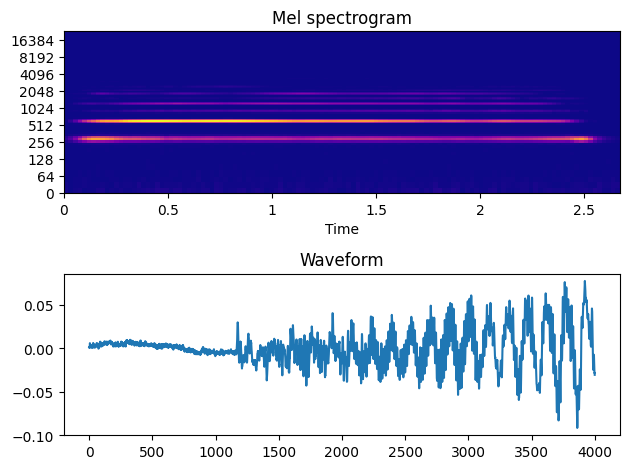
\includegraphics[width=0.7\linewidth]{rys06/target_sample_flute_literature.png}
    \caption{
      Spektrum fouriera i współczynniki MFCC dla dźwięku \texttt{flute.wav} wykorzystywanego
      do eksperymentów w~\cite{evolutionary_puredata_results}.
    }\label{fig:literature_flute_sound_overview}
\end{figure}

Dźwięk \texttt{flute\_.wav}~(\ref{fig:literature_flute_sound_overview})
jest nagraniem prawdziwego instrumentu dętego. Kształt fali jest nieregularny,
charakterystyka spektralna zawiera dynamicznie pojawiające się i słabnące 
składowe częstotliwościowe.

\subsection{Sampel z syntezatora \textit{OP-1}}

Dźwięk \texttt{op1\_1.wav}, wygenerowany przy pomocy syntezatora \textit{OP-1} jest próbą
zasymulowania dźwięku instrumentu dętego.

\begin{figure}[H]
    \centering
    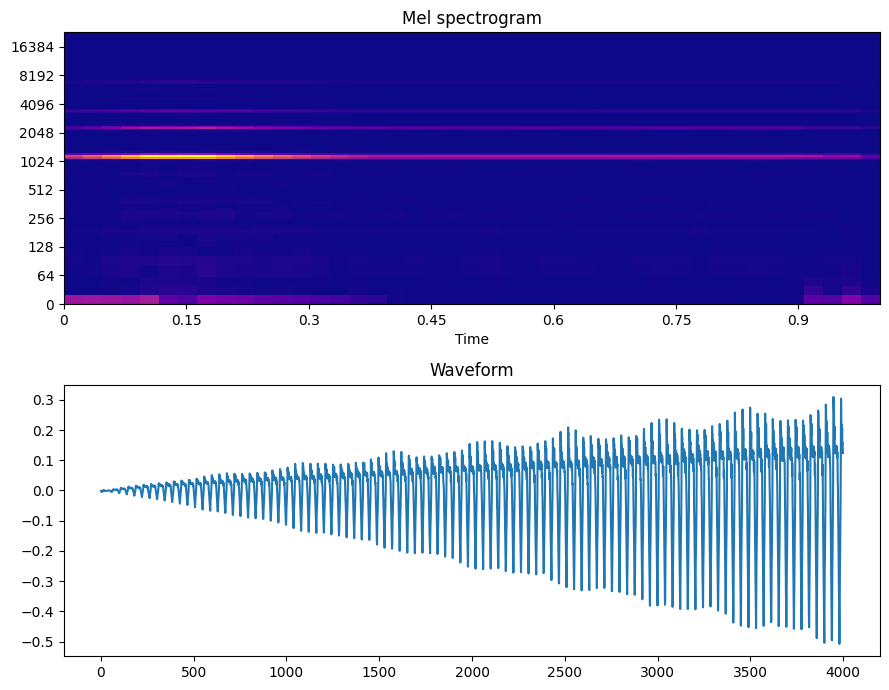
\includegraphics[width=0.7\linewidth]{rys06/target_sample_op1_literature.png}
    \caption{
      Spektrum fouriera i współczynniki MFCC dla dźwięku \texttt{op1\_1.wav} wykorzystywanego
      do eksperymentów w~\cite{evolutionary_puredata_results}.
    }\label{fig:literature_op_1_sound_overview}
\end{figure}

\subsection{Transjent}

Dźwięk \texttt{transient.wav}, przedstawiony na rysunku~\ref{fig:literature_transient_sound_overview},
został wykorzystany w literaturze~\cite{evolutionary_puredata} do sprawdzenia jak dobrze algorytm
generujący dźwięk potrafi przybliżyć dźwięki o dynamicznych zmianach w charakterystyce spektralnej.
Tego typu dźwięki są typowe dla instrumentów takich jak fortepian lub klawesyn.

\begin{figure}[H]
    \centering
    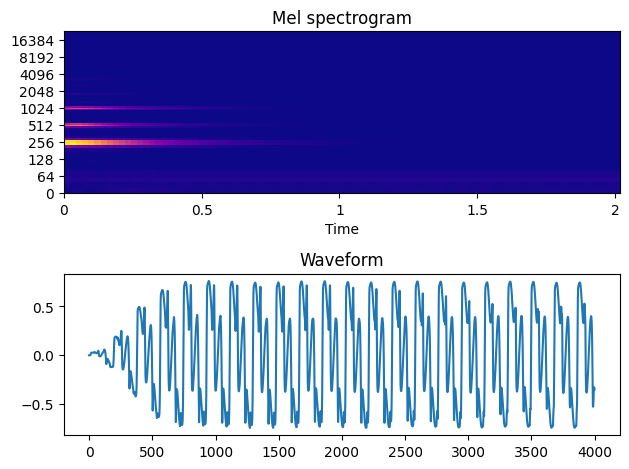
\includegraphics[width=0.7\linewidth]{rys06/transient_sample_literature.png}
    \caption{
      Spektrum fouriera i współczynniki MFCC dla dźwięku \texttt{transient.wav} wykorzystywanego
      do eksperymentów w~\cite{evolutionary_puredata_results}.
    }\label{fig:literature_transient_sound_overview}
\end{figure}



